%! TEX root = **/010-main.tex
% vim: spell spelllang=ca :

% DESCRIPTORS
% RegionProps -> Circularity
%


%- Justificació del descriptors utilitzats i procediment d'obtenció.
%- Descripció de les rutines utilitzades, tant les implementades pels estudiants com les contribuïdes per altres
%- Classificador que s'utilitzarà. Motius.
%- Resultats preliminars (si n'hi ha algun)


\section{Preprocessat}

Per poder processar les imatges i obtenir els indicadors, primerament utilitzarem
diverses rutines de MATLAB per tal de millorar el color i contrast de les imatges per tenir
imatges mes homogènies i poder separar els colors mes fàcilment.

Després de revisar les imatges per sobre vam veure que moltes tenien problemes de
i\lgem uminació. Per tal de solucionar aquest inconvenient vam decidir per ús d'una
tècnica anomenada \emph{haze removal}, o eliminació de boira en català, que permet
millorar la i\lgem uminació.

Les imatges amb poca i\lgem uminació tenen en comú amb les imatges emboirades que el
histograma de la imatge inversa és molt semblant. Per tant, podem invertir la imatge,
aplicar-li el procés de \emph{haze removal} (fent ús de la funció de MATLAB 
\texttt{imreducehaze}) i tornar a invertir la imatge.  Aquest procés es pot
apreciar en la figura \cite{fig:preprocess_montage}. Com podem veure, al invertir la
imatge les parts més fosques passen a tenir una boira blanquinosa que el
\texttt{imreducehaze} elimina a la tercera imatge.

\begin{figure}[H]
\centering
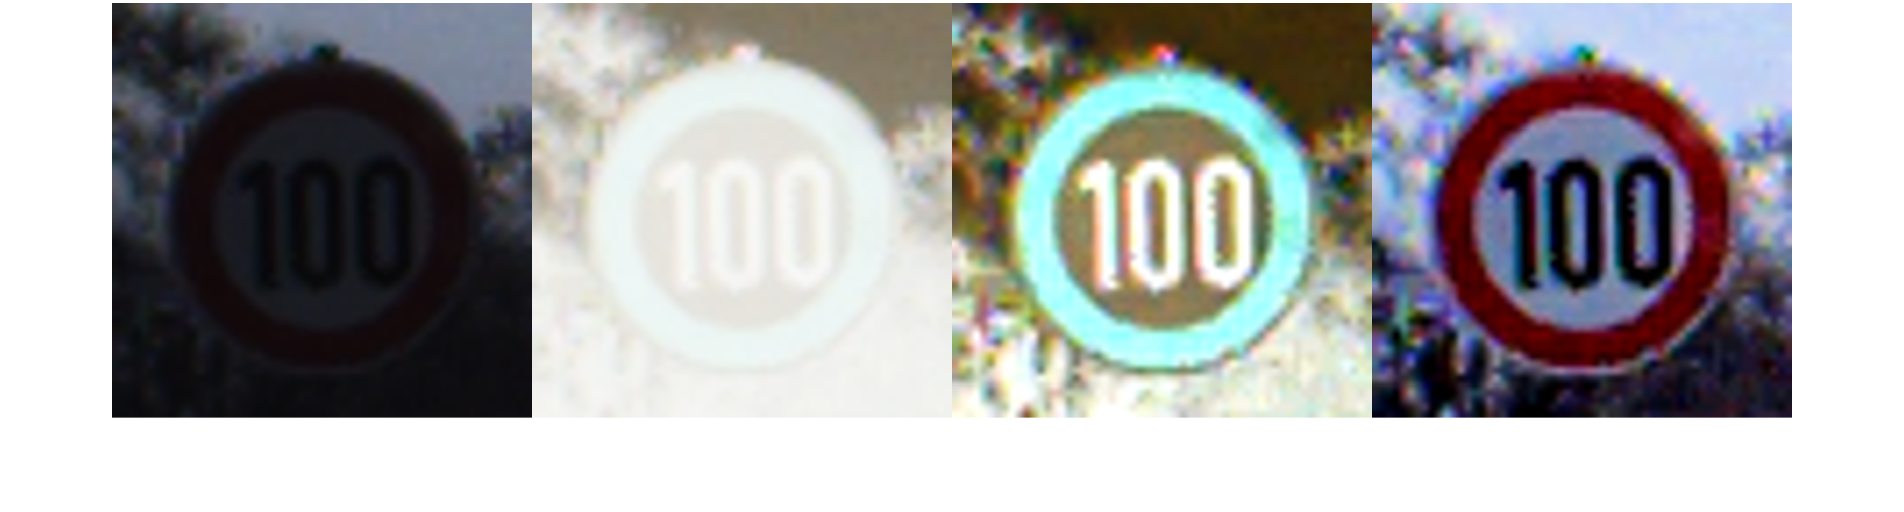
\includegraphics[width=0.9\textwidth]{preprocess_montage}
\caption{Passos intermedis del pre-processat}%
\label{fig:preprocess_montage}
\end{figure}

Una imatge amb boira $I$ es poden modelar de la següent forma:

$$I = J \cdot T + L(1-T)$$

On $J$ és la imatge sense boira, $T$ és un mapa de transmissió de la llum i
$L$ és la boira.

\texttt{imreducehaze} agafa la imatge emboirada $I$ i estima $L$, amb Dark Channel Prior,
i $T$ per poder
aproximar $J$. A més, en el nostre cas li passem la opció \emph{ContrastEnhancement}
amb valor \emph{boost} per millorar el contrast també.

A l'\cref{app:pre} hi ha el codi del pre-processat en detall.
